%!TEX TS-program = xelatex
\documentclass{beamer}

\usepackage[linesnumbered,lined,boxed,commentsnumbered]{algorithm2e}

%%% Работа с русским языком и шрифтами
\usepackage[english,russian]{babel}   % загружает пакет многоязыковой вёрстки
\usepackage{fontspec}      % подготавливает загрузку шрифтов Open Type, True Type и др.
\defaultfontfeatures{Ligatures={TeX},Renderer=Basic}  % свойства шрифтов по умолчанию
\setmainfont[Ligatures={TeX,Historic}]{Myriad Pro} %  установите шрифты Myriad Pro или (при невозможности) замените здесь на другой шрифт, который есть в системе — например, Arial
\setsansfont{Myriad Pro}  %  установите шрифты Myriad Pro или (при невозможности) замените здесь на другой шрифт, который есть в системе — например, Arial
\setmonofont{Courier New}
\uselanguage{russian}
\languagepath{russian}
\deftranslation[to=russian]{Theorem}{Теорема}
\deftranslation[to=russian]{Definition}{Определение}
\deftranslation[to=russian]{Definitions}{Определения}
\deftranslation[to=russian]{Corollary}{Следствие}
\deftranslation[to=russian]{Fact}{Факт}
\deftranslation[to=russian]{Example}{Пример}
\deftranslation[to=russian]{Examples}{Примеры}

\usepackage{multicol} 		% Несколько колонок
\graphicspath{{images/}}  	% Папка с картинками
\usepackage{subcaption}

\usepackage{hyperref}
\urlstyle{same}

%%% Информация об авторе и выступлении
\title[Заголовок]{Графовые свёрточные нейронные сети} 
% \subtitle{Подзаголовок презентации / Название конференции}
\author[Александр Колодезный]{Александр Колодезный БПМИ192}
\institute[Высшая школа экономики]{Национальный исследовательский университет \\ «Высшая школа экономики» (Москва)}
\date{23 ноября 2021 г.}

\begin{document}	% Начало презентации

\frame[plain]{\titlepage}	% Титульный слайд

\begin{frame}
\frametitle{Graph Convolutional Network}
Вид одного слоя
\begin{figure}
	% 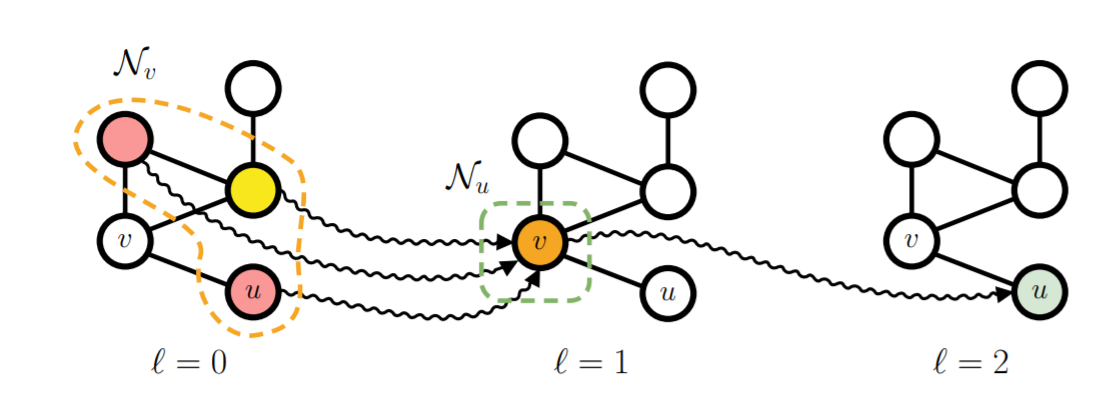
\includegraphics[width=\columnwidth]{message_propagation.png}
	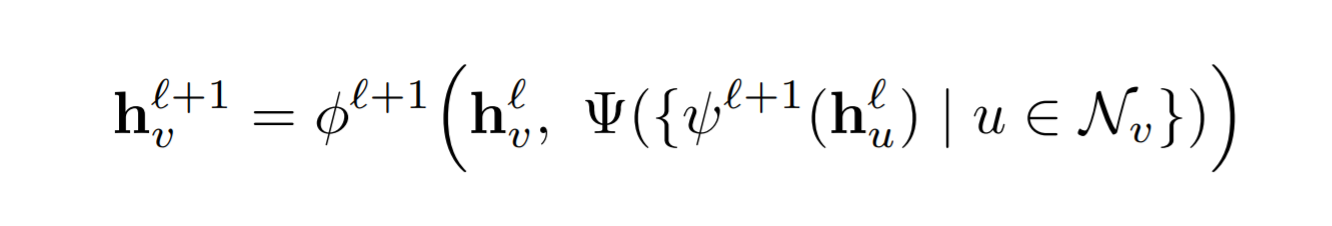
\includegraphics[width=\columnwidth]{fromula1.png}
\end{figure}
\begin{itemize}
	\item $\Psi$ --- permutation-invariant функция
	\item $\phi^{l + 1}$ и $\psi^{l + 1}$ --- некоторый функция на $l$-ом слое
\end{itemize}
\end{frame}

\begin{frame}
\frametitle{Graph Convolutional Network}
\begin{figure}
	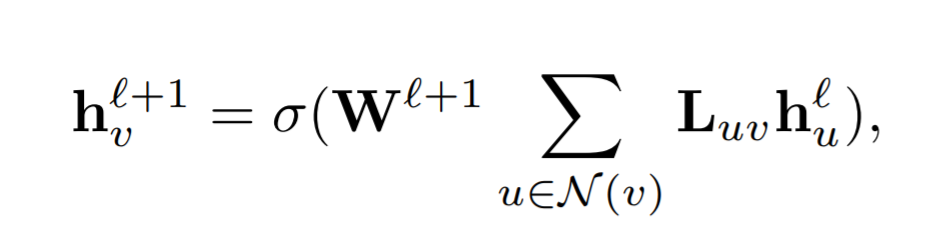
\includegraphics[width=0.8\columnwidth]{formula2.png}
\end{figure}
\begin{itemize}
	\item $\sigma$ --- сигмоида
	\item $W^{l + 1}$ --- обучаемая матрица
	\item $L_{uv}$ --- нормированный Лаплассиан
\end{itemize}
\end{frame}

\begin{frame}
\frametitle{Sampling}
\begin{multicols}{2}
Виды
\begin{itemize}
	\item Для каждой вершины выбираем случайное подмножество соседних, которые будут влиять на новое значение $h_v$. (GraphSAGE).
	\item Выбирать случайное множество вершин всего графа и обучаться только на полученном ими подграфе (FastGCN).
\end{itemize}
	
\columnbreak
	\begin{figure}
		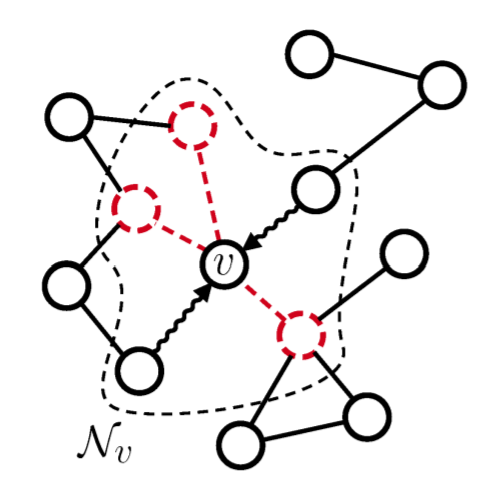
\includegraphics[width=\columnwidth]{sampling.png}
	\end{figure}
\end{multicols}
\end{frame}

\begin{frame}
\frametitle{Pooling}
\begin{figure}
	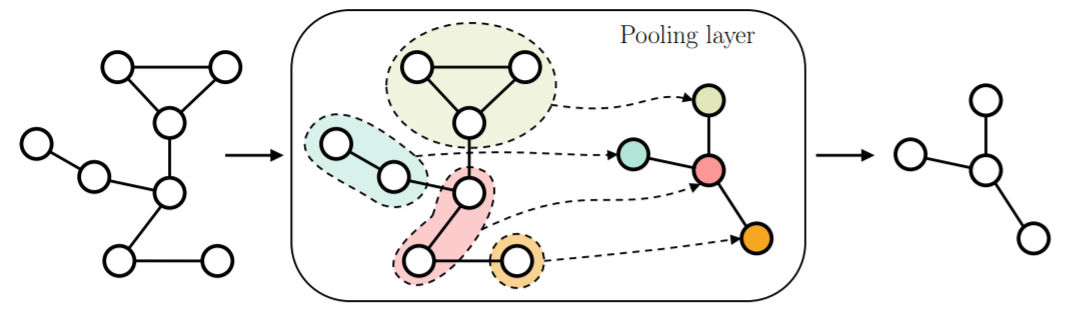
\includegraphics[width=\columnwidth]{pooling.png}
\end{figure}
\begin{itemize}
	\item Сжатие кластеров вершин в одну
	\item Уменьшает размеры графа
	\item Уменьшает вычислительную стоимость
\end{itemize}
\end{frame}

\begin{frame}
\frametitle{Differentiable Pooling}
\begin{itemize}
	\item Обучаем для каждой вершины попадание в кластера
\begin{figure}
	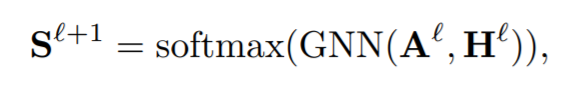
\includegraphics[width=0.5\columnwidth]{softmax.png}
\end{figure}
	\item Пересчитываются embedding для новых вершин, и новая матрица смежности
	\begin{figure}
		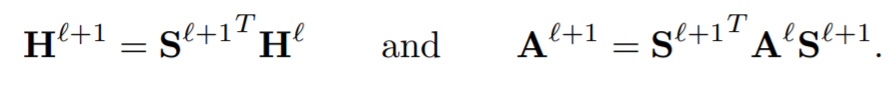
\includegraphics[width=0.8\columnwidth]{differentaible_pooling.png}
	\end{figure}
	\item Новая матрица смежности оказывается полной
\end{itemize}
\end{frame}

\begin{frame}
\frametitle{Top-k Pooling}
\begin{itemize}
	\item Для каждой вершины посчитаем attention как проекция его эмбединга на обучаемый вектор $p$
	\begin{figure}
		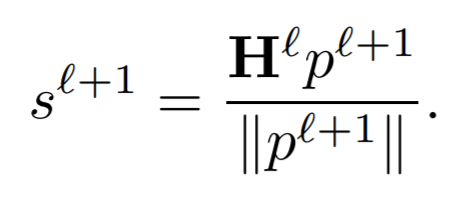
\includegraphics[width=0.3\columnwidth]{top-k_pooing.png}
	\end{figure}
	\item Выбираем $k$ вершин с наибольшим полученным attention
	\item Оставляем м графе только найденные вершины
	\item Расширение метода Self-attention pooling
	\begin{figure}
		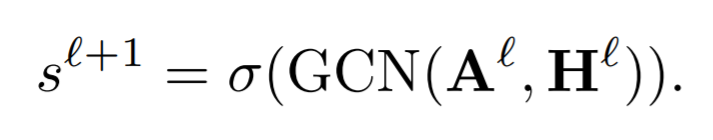
\includegraphics[width=0.5\columnwidth]{self-attention_pooing.png}
	\end{figure}
\end{itemize}
\end{frame}

\begin{frame}
\frametitle{Другие методы pooling-а}
\begin{itemize}
	\item Edge pooling --- выбираем ребро, которое сжимаем
	\begin{figure}
		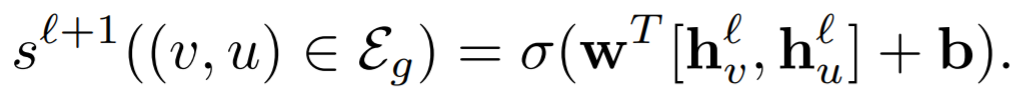
\includegraphics[width=0.7\columnwidth]{edge_pooling.png}
	\end{figure}
	\item Топологические виды pooling-а
	\begin{itemize}
		\item GRACLUS --- алгоритм основанный на спектральной кластеризации
		\item Non-negative Factorization Matrix Pooling --- pooling основанный на NFM факторизации матрицы смежности.
	\end{itemize}
\end{itemize}
\end{frame}

\begin{frame}
\frametitle{Graph embedding}
\begin{itemize}
	\item Хотим построить embedding для всего графа
	\item Нужно агрегировать embedding для нод
	\item Можно делать polling графа, пока не останется одна вершина
	\item Применить перестановочно-инвариантную функцию от всех нод
	\begin{figure}
		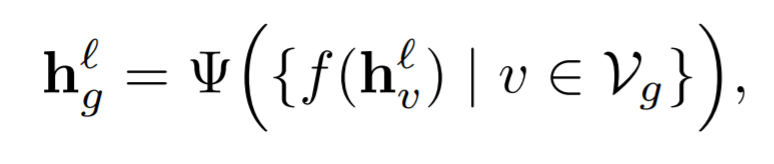
\includegraphics[width=0.5\columnwidth]{graph_classification.png}
	\end{figure}
	\item Выбрать $\Psi$ как сумму, максимум или минимум, а $f$ --- тождественную функцию.
\end{itemize}
\end{frame}

\begin{frame}
\frametitle{Список литературы}
\begin{itemize}
	\item \url{https://arxiv.org/pdf/1912.12693.pdf}
	\item \url{https://arxiv.org/pdf/1609.02907.pdf}
	\item \url{https://arxiv.org/pdf/1812.04202.pdf}
	\item \url{https://arxiv.org/pdf/1801.10247.pdf}
	\item \url{https://arxiv.org/pdf/1706.02216.pdf}
\end{itemize}
\end{frame}



% \begin{frame}[c]
% \begin{center}
% \frametitle{\LARGE Спасибо за внимание!}

% {\LARGE \inserttitle}

% \bigskip

% {\insertauthor} 

% \bigskip\bigskip

% {\insertinstitute}

% \bigskip\bigskip

% {\large \insertdate}
% \end{center}
% \end{frame}

\end{document}